
\chapter[Appendix C]{Appendix C}

%~~~~~~~~~~~~~~~~~~~~~~~~~~~~~~~~~~~
%~~~~ C.1. Survey Information
%~~~~~~~~~~~~~~~~~~~~~~~~~~~~~~~~~~~
\section[The Boko Haram Survey]{The Boko Haram Survey}
\label{app:C1}

%~~~~~~~~~~~~~~~~~~~~~~~~~~~~~~~~~~~
\subsection{A Three-Stage Sampling Process}
%~~~~~~~~~~~~~~~~~~~~~~~~~~~~~~~~~~~
In 2014, the Centre for Research on Peace and Development (CRPD) at the University of Leuven (KU Leuven) set up a large-scale longitudinal panel study with Nigerian university students in order to evaluate the extent to which the National Youth Service Corps (NYSC) contributed to improved intergroup relations and stronger national identities (see Schroyens, \citeyear{Schroyens2019}, for more information on this evaluation project).\footnote{In general, this section on sampling has greatly benefited from the doctoral thesis of Maarten Schroyens (\citeyear{Schroyens2019}). Thanks!} When this project was finished, the panel was updated and contacted again to participate in a new project unraveling public opinion on the Boko Haram (BH) insurgency. In the remainder of this text, the original evaluation project is referred to as ``NYSC survey'', while the data in the manuscript comes from the ``BH Survey''. In what follows, we explain the three-stage sampling mechanism used to sample the respondents. Our sampling procedure largely builds on the insights gained by Langer and colleagues (\citeyear{Langer2017a}).


Although the importance and application of large-scale surveys in developing countries is growing, contextual factors continue to confront survey researchers with a series of pressing methodological and practical challenges \citep{Bulmer1993, Bulmer1993b}. One particular challenge to recruit respondents for the initial NYSC survey was the absence of a reliable sampling frame. Both the Nigerian universities and the NYSC secretariat informed us that they could only provide the names of their students or prospective participants, respectively, but not their contact details. We therefore implemented a multistage sampling mechanism. In the first stage (see Figure \ref{fig:art2-app-fig1}), students from a diverse array of randomly selected Bachelor programs in a number of purposefully selected universities were recruited by means of an off-line paper-administered self-interview (PASI). Five federal universities were selected to be included in study: the University of Nigeria (UNN) in Nsukka, University of Abuja, University of Lagos, Usmanu Danfodiyo University (UDU) in Sokoto, and University of Port-Harcourt. These universities guaranteed an ethno-regional and -religious mix of students while simultaneously took into account safety precautions. Unfortunately, our university did not grant us permission to select a North-Eastern university due to security concerns. Official permission to survey the students was obtained from the central University Administration. The classes were visited in May-September 2015, and the in-class survey of 12–15 minutes was usually conducted at the beginning or ending of a lecture. The main goals of this in-class survey were to (1) obtain email addresses and phone numbers to create an online panel and (2) build trust as to the sincerity, relevance, and political independence of our project. A total of 6,830 students across the five universities completed this in-class questionnaire.

%~~~~~~~~~~~~~~~~~~~~~~~~~~~~~~~~~~~
% Figure C.1
%~~~~~~~~~~~~~~~~~~~~~~~~~~~~~~~~~~~
\vspace{1.5mm}
\begin{figure}[H]
\centering
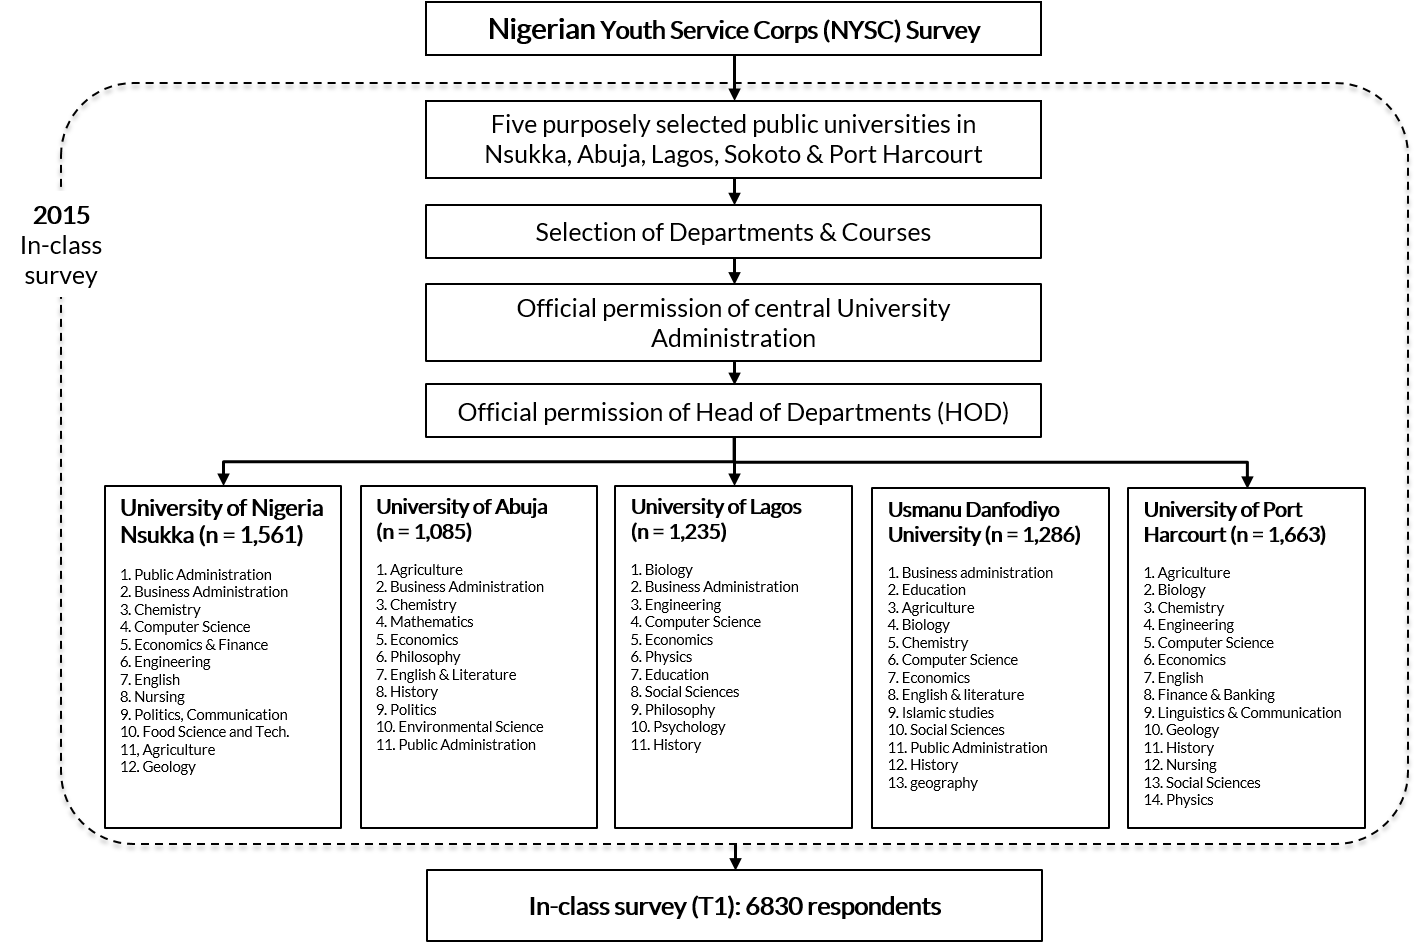
\includegraphics[width=\textwidth]{Appendices/Appendix_chapter_3/art2-app-figure1.png}
\caption{First Stage of the Sampling Process}
\label{fig:art2-app-fig1}    
\end{figure}
%~~~~~~~~~~~~~~~~~~~~~~~~~~~~~~~~~~~

In the second stage (see Figure \ref{fig:art2-app-fig2}), using the contact information respondents provided during the in-class survey, the students were invited to participate in a web self-administered questionnaire  \citep[WSAQ;][]{Callegaro2015}. There were a several reasons why we chose to employ a WSAQ. First, the target population was widely dispersed and highly mobile, and a WSAQ allowed us to keep track of our participants. Second, given the relatively sensitive nature of various topics addressed in the survey (e.g., inter-ethnic and -religious relations, corruption, political violence, ...), an interviewer-mediated approach could increase social desirability biases \citep{DuToit2016}. Third, the cost effectiveness of WSAQ surveys allowed for a larger sample size within the available budget. A convenient byproduct is that a WSAQ enabled us to conduct the conjoint experiment in the 2018 wave.\footnote{The conjoint experiment required an internet connection because, each time a respondent reached the experiment, Qualtrics recalled a PHP script hosted on a server to randomize the attributes. These randomized attributes then got piped back into an HTML-created 2*7-table in Qualtrics.} 


The first online survey took place before the students went for national service (Oct. 2015--Febr. 2016), the second one after they finished their service (April or Aug.--Sept. 2017, depending on the batch in which the students were sent out for service). Students were invited to participate in the online surveys by email, while text messages were also sent to respondents’ mobile phones informing them about the invitation and incentive they receive after participation. Via text messages, 921 missing or wrong e-mail addresses were retrieved. Reminders to participate were sent after one, two, and three weeks again both by email and text message. A total of 2,585 students completed the first online questionnaire (plus 720 partial completions), while 2,302 respondents competed the second online questionnaire (plus 135 partial completions).

%~~~~~~~~~~~~~~~~~~~~~~~~~~~~~~~~~~~
% Figure C.2
%~~~~~~~~~~~~~~~~~~~~~~~~~~~~~~~~~~~
\vspace{3mm}
\begin{figure}[H]
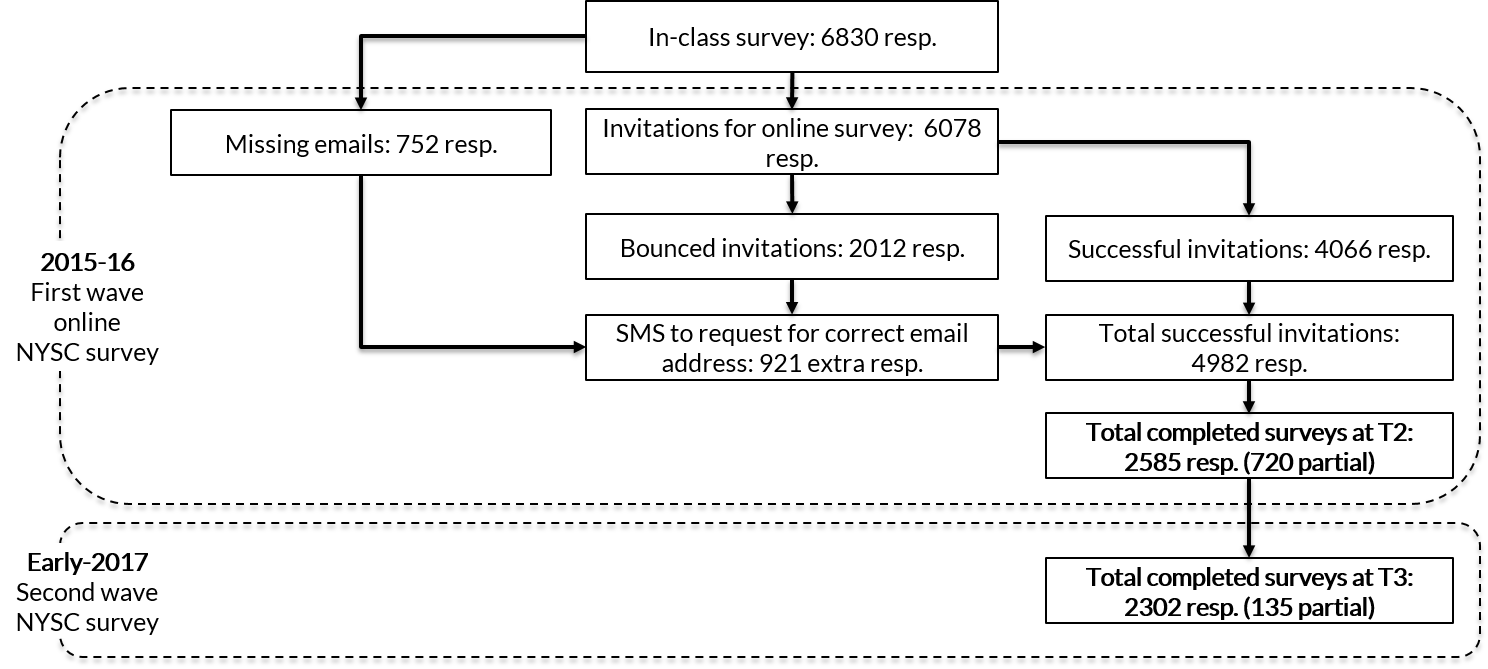
\includegraphics[width=1\textwidth]{Appendices/Appendix_chapter_3/art2-app-figure2.png}
\caption{Second Stage of the Sampling Process}
\label{fig:art2-app-fig2}
\end{figure}
%~~~~~~~~~~~~~~~~~~~~~~~~~~~~~~~~~~~

In 2017, the project evaluating the NYSC terminated, while another research project on the impact of the Boko Haram violence commenced. Given the unique access we gained in the years before, we decided to update all contact information and to re-contact the original sample. We had three sources of information to update our contact entries. Each year, after completion of the study, participants were asked to leave their phone number in order to receive their phone top-ups. They could also leave their (new) e-mail address at the end of the survey. Last, several respondents contacted us throughout the years to inform us that they had a new e-mail address or phone number. This strategy left us with 6,199 e-mail addresses that were re-contacted in November 2017. A total of 2,492 students completed the 2017 survey (plus 92 partial completions), while 2,124 students completed the 2018 survey (plus 31 partial completions).

%~~~~~~~~~~~~~~~~~~~~~~~~~~~~~~~~~~~
% Figure C.3
%~~~~~~~~~~~~~~~~~~~~~~~~~~~~~~~~~~~
\vspace{3mm}
\begin{figure}[H]
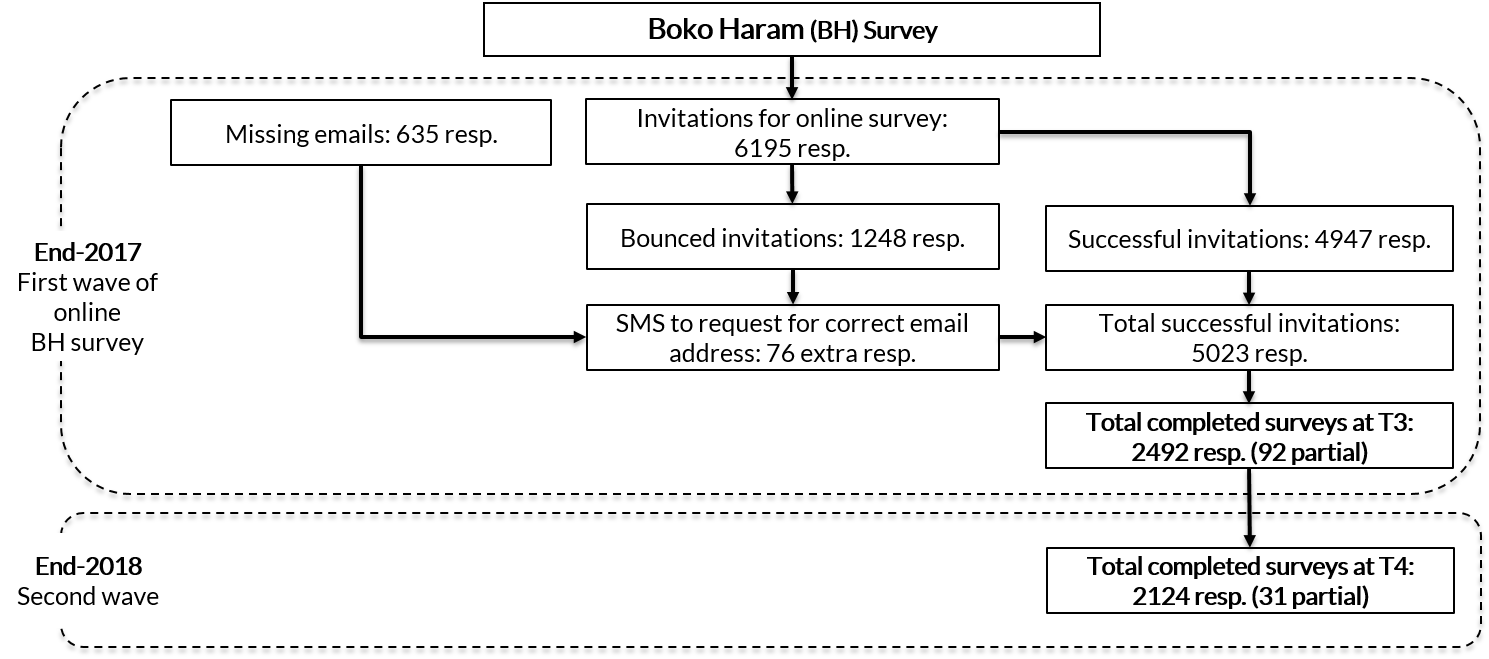
\includegraphics[width=1\textwidth]{Appendices/Appendix_chapter_3/art2-app-figure3.png}
\caption{Third Stage of the Sampling Process}
\label{fig:art2-app-fig3}
\end{figure}
%~~~~~~~~~~~~~~~~~~~~~~~~~~~~~~~~~~~


%~~~~~~~~~~~~~~~~~~~~~~~~~~~~~~~~~~~
\subsection{Response and Attrition Rates}
%~~~~~~~~~~~~~~~~~~~~~~~~~~~~~~~~~~~
\subsubsection{Maximizing Response Rates}
\label{app:C12}
%~~~~~~~~~~~~~~~~~~~~~~~~~~~~~~~~~~~
To maximize the response rate and minimize the attrition rate, we followed several recommendations as set out in the Tailored Design Method \citep[TDM;][]{Dillman1978, Dillman2014} and by Langer, Meuleman, and colleagues (\citeyear{Langer2017a, Meuleman2018}). First, we sent invitations and reminders via both e-mail and text messages. Using text messaging proved to be a crucial component to reach the target population as several e-mail addresses bounced back the first time. Second, reminders were sent after one, two, and three weeks (again via e-mail and text messages). The survey usually closed after 28 days. Third, time investment was minimized by keeping the survey as short as possible, while a clear and minimal layout was used to facilitate comprehension of the question. This latter strategy was also important to minimize the time needed to load a survey page as bandwidth in Nigeria is more limited. Fourth, for each online survey, respondents were offered a monetary incentive conditional on completion of the survey. Because direct cash incentives were not feasible, we gave respondents a mobile top-up of 1,500 naira (i.e., about 4\$). Our preparatory fieldwork confirmed that mobile phone credits function as an easily transmittable quasi-cash incentive in Nigeria, given that our students informed us that mobile phones credited via a pay-as-you-go system are widely used. Mobile top-ups were sent using the electronic payment platform from E-tranzact, which allowed us to distribute top-ups to all phone providers in Nigeria.


%~~~~~~~~~~~~~~~~~~~~~~~~~~~~~~~~~~~
\subsubsection{Response and Attrition Rates}
%~~~~~~~~~~~~~~~~~~~~~~~~~~~~~~~~~~~
In what follows, several response rates are calculated using AAPOR guidelines \citep{AAPOR2016}. Almost 40\% of the baseline in-class sample completed the first online survey (i.e., the minimum response rate or RR1 = $\frac{2,585}{6,830}$ = 37.8\%). This number gives a rather pessimistic estimation, however, since we encountered a relatively a higher number of bounced emails and failed text messages. When taking non-contact into account, the so-called minimum cooperation rate (COOP1) constitutes 51.9\% (i.e. 2,585 complete responses divided by all 4,982 eligible units ever contacted). When also considering partial responses, the cooperation rate further increases to 66.8\% (i.e., 3,305 fully and partially completed responses divided by 4,982 contacted students). The completion rate for the first online survey is 78.2\% (i.e., $\frac{2,585}{3,305}$). Table \ref{tab:art2-app-tab1} checks whether some respondents were significantly more likely to participate in the online survey by comparing the minimum cooperation rates by gender, religion, and university for the first online survey. As one can see, men, Christians, and students from the University of Lagos were more likely to participate in the online survey (probably because of better access to the internet). 


After we updated and re-contacted the sample, 40.2\% (i.e., 2,492 surveys completed divided by 6,195 invited students) respondents fully completed the 2017 online survey, which increases to 49.6\% if you take into account the number of bounced emails (i.e., 2,492 complete responses divided by 5,023 eligible units contacted) and to 51.5 \% if you also consider the partial completions (i.e., 2,584 fully and partially completed responses divided by 5,023 contacted students). The completion rates in these last two surveys are remarkably high (i.e., 96.3\% and 99\%), which suggests that respondents are quite interested in the topic of this new project. Table \ref{tab:art2-app-tab2} summarizes the number of complete and partial responses in all survey waves. Last, on average, the item non-response across survey waves for all questions was 2.5\%, which is similar to results from Western web-based surveys \citep{Lesser2012, Millar2012}.


%~~~~~~~~~~~~~~~~~~~~~~~~~~~~~~~~~~~
% Table C.1
%~~~~~~~~~~~~~~~~~~~~~~~~~~~~~~~~~~~
\vspace{3mm}
\begin{table}[H]
\caption{Cooperation Rates by Gender, Religion, and University for First Online Survey}
\label{tab:art2-app-tab1}
\onehalfspacing
\resizebox{\textwidth}{!}{%
\begin{tabular}[c]{@{}llccccc@{}}
\toprule
\midrule
 & & \multicolumn{2}{c}{No/Partial response} & \multicolumn{2}{c}{Complete response} & $\chi^2$-test \\ \midrule
\multicolumn{2}{l}{Total} & 2,397 & 48.1\% & 2,585 & 51.9\% &  \\
\multicolumn{2}{l}{Gender} &  &  &  &  & $\chi^2(1)$ = 27.076, $p<.001$ \\
 & Male & 1,237 & 44.8\% & 1,527 & 55.2\% &  \\
 & Female & 1,148 & 52.2\% & 1,052 & 47.8\% &  \\
\multicolumn{2}{l}{Religion} &  &  &  &  & $\chi^2(2)$ = 8.805, $p=.012$ \\
 & Christian & 1,796 & 47.5\% & 2,010 & 52.8 \% &  \\
 & Muslim & 504 & 52.5\% & 456 & 47.5\% &  \\
 & Other/No & 61 & 50.0\% & 61 & 50.0\% &  \\
\multicolumn{2}{l}{University} &  &  &  &  & $\chi^2(4)$ = 78.638, $p<.001$ \\
 & Nsukka & 568 & 46.7\% & 647 & 53.3\% &  \\
 & Abuja & 415 & 53.2\% & 365 & 46.8\% &  \\
 & Lagos & 378 & 37.1\% & 640 & 62.9\% &  \\
 & Sokoto & 445 & 55.5\% & 357 & 44.5\% &  \\
 & Port-Harcourt & 591 & 50.6\% & 576 & 49.4\% &  \\ \midrule \bottomrule
\end{tabular}%
}
\end{table}
%~~~~~~~~~~~~~~~~~~~~~~~~~~~~~~~~~~~


%~~~~~~~~~~~~~~~~~~~~~~~~~~~~~~~~~~~
% Table C.2
%~~~~~~~~~~~~~~~~~~~~~~~~~~~~~~~~~~~
\vspace{3mm}
\begin{table}[H]
\caption{Overview of Sample Size Across Survey Waves}
\label{tab:art2-app-tab2}
\onehalfspacing
\resizebox{\textwidth}{!}{%
\begin{tabular}{@{}p{3.5cm}>{\centering\arraybackslash}p{1.8cm}>{\centering\arraybackslash}p{1.8cm}>{\centering\arraybackslash}p{1.8cm}>{\centering\arraybackslash}p{1.8cm}>{\centering\arraybackslash}p{1.8cm}@{}}
\toprule
\midrule
                    & Offline          & \multicolumn{2}{c}{NYSC Online Survey}    & \multicolumn{2}{c}{BH Online Survey}  \\
                    & Baseline         & \multicolumn{2}{c}{($N=4,982$ contacts)} & \multicolumn{2}{c}{($N=5,022$ contacts)}\\
                    & 2015             & 2015-16        & Early-2017                    & End-2017       & End-2018 \\ \midrule
All responses       & 6,630            & 3,305          & 2,437                     & 2,584     & 2,155  \\ 
Complete responses  & 6,630            & 2,585          & 2,302                     & 2,492     & 2,124  \\ 
Partial responses   & NA               & 720            & 135                       & 92        & 31  \\ \midrule \bottomrule
\end{tabular}%
}
\end{table}
\newpage


%~~~~~~~~~~~~~~~~~~~~~~~~~~~~~~~~~~~
\subsection{Survey Items}
\label{app:C13}
%~~~~~~~~~~~~~~~~~~~~~~~~~~~~~~~~~~
Below, we provide the exact question wording and response options for the covariates used in the paper. These questions were measured in the 2017 online wave of the Boko Haram survey, while the conjoint experiment was conducted in the 2018 wave.

\begin{mdframed}
\begin{table}[H]
\setstretch{1.1}
\begin{tabular}{lp{9.6cm}}
\multicolumn{2}{l}{\textbf{Covariate 1. Religion}} \\
Question wording   & What is your religion?  \\
Response options   & \tabitem Christianity \\
                   & \tabitem Islam \\
                   & \tabitem Traditional African religion \\
                   & \tabitem No religion \\
                   & \tabitem Other religion, please specify: [open text box] \\ [2ex]
\multicolumn{2}{l}{\textbf{Covariate 2. Exposure to BH Violence}} \\
Question info      & Exposure to terrorism was measured by asking respondents whether they had been exposed to the incidents stated below. Respondents who were exposed to at least one incident were coded as 1, respondents who were exposed to none as 0. \\
Question intro     & The Boko Haram crisis has had a major impact on Nigeria. We are interested in how it has affected your life. \\
Questions          & Have you ever personally witnessed a violent attack by Boko Haram? \\
                   & Has anyone of your family or friends ever witnessed a violent attack by Boko Haram?\\
                   & Have you ever been personally injured in a violent attack by Boko Haram?\\
                   & Has anyone of your family or friends ever been injured in a violent attack by Boko Haram?\\
                   & Have you lost anyone of your family or friends in a violent attack by Boko Haram?\\
                   & Have you ever experienced any loss of employment or income because of a violent attack by Boko Haram?\\ 
Response options   & \tabitem Yes \tabitem No \\ [2ex]
\multicolumn{2}{l}{\textbf{Covariate 3. Anger Reactions to BH Violence}} \\
Question info       & Anger was one of six emotions asked. The other emotions were sadness, guilt, pride, anger, fear, and shame. \\
\end{tabular}
\end{table}
\end{mdframed}

\begin{mdframed}
\begin{table}[H]
\setstretch{1.1}
\begin{tabular}{lp{9.6cm}}
Question intro      & Thinking about the Boko Haram crisis, to what extent do you feel the following emotions on a scale from 0 (= not at all) to 10 (= very much)? \\
                    & You can choose any number between 0 and 10. Choosing a lower number indicates that you feel this emotion less when thinking about Boko Haram. Choosing a higher number indicates that you feel this emotion more when thinking about Boko Haram.\\
Question wording    & Anger \\
Response options    & 0 (not angry at all) - 1 - 2 - 3 - 4 - 5 - 6 - 7 - 8 - 9 - 10 (very angry) \\
\end{tabular}
\end{table}
\end{mdframed}


%~~~~~~~~~~~~~~~~~~~~~~~~~~~~~~~~~~~
%~~~~~ Quantities of Interest 
%~~~~~~~~~~~~~~~~~~~~~~~~~~~~~~~~~~~
\section{Quantities of Interest}
\label{app:C2}
%~~~~~~~~~~~~~~~~~~~~~~~~~~~~~~~~~~~
\subsection[Interpretation]{Interpretation\footnote{This section hugely benefited from and applies the notation used in the Supplementary Information provided by Thomas Leeper, Sara Hobbolt, and James Tilley in their \citeyear{Leeper2019} Political Analysis article.}}
\label{app:C21}
%~~~~~~~~~~~~~~~~~~~~~~~~~~~~~~~~~~~
The \textit{average treatment effect} (ATE) is probably one of the most common quantity of interest within experimental designs \citep{Gerber2012} and, in the context of conjoint experiments, represents the difference in responses (or cell means, $E[Y\mid\overrightarrow{\rm X} = \overrightarrow{\rm x}]$) for two different sets of profiles. Estimating this quantity is an unfeasible task considering that the number of observations in a typical conjoint experiment is much lower the number of possible profiles ($N<C$). In other words, the means for many --and often for most-- experimental cells remain unobserved. In our experiment, assuming full randomization, there are 43,200 possible profiles while we have 11,580 rated profiles clustered within 1,930 respondents, so more than 70 percent of all experimental cells remain unobserved ($N \ll C$). Fortunately, the main strength of a conjoint experiment is that it enables estimating an alternative quantity of interest, being the \textit{average marginal component effect} \citep[AMCE;][]{Hainmueller2014a}. AMCEs quantify the overall effect of an individual treatment component (or feature) rather than the effect of an entire set of components given that, in most conjoint experiments, $N > F$. Formally, AMCEs are defined as the marginal effect of a certain attribute averaged over the joint distribution of the remaining attributes (or, in other words, differences in conditional/marginal means, $E[Y\mid\overrightarrow{\rm X_{f}} = \overrightarrow{\rm x_{f}} ]$). While a comparison of marginal means allows \textit{causal} interpretation of conjoint experiments, Leeper and colleagues (\citeyear{Leeper2019}) shown how the marginal means alone are of direct interest for the common \textit{descriptive} use of conjoint designs. \textit{Marginal Means} (MMs) are defined as the  ``favorability on the scale of the outcome over alternative values of each feature independent of the features in the design'' \citep[][, SI p.5]{Leeper2019}. As we explain in the main article, the difference between marginal means (MMs) and a comparison of marginal means (AMCEs) becomes especially important when estimating heterogeneous treatment effects--a key quantity of interest in our study.

Noteworthy, Abramson, Kocak, and Magazinnik (\citeyear{Abramson2019}) recently demonstrate how conjoint experiments (and more specifically, AMCEs and MMs) do not capture the underlying majority preference, but they are often interpreted as doing so. In other words, conjoints do not reflect preferences in the strict economic sense of the term. This is not a consequence of uncertainty or bias, but is inherent to the AMCEs properties as an aggregation mechanism. More specifically, AMCEs and, by extension, MMs are influenced by both preference \textit{direction} (i.e., what feature respondents prefer) and preference \textit{intensity} (i.e., how much weight respondents give to that feature's attribute relative to the other attributes). For example, imagine that a majority of voters has a \textit{weak} preference for a male candidate, whereas a minority of voters has a \textit{strong} preference for a female candidate. This minority will therefore always prefer a female candidate over a male candidate (e.g., even when a female candidate does not align with the respondent's own party identity), while the majority will sometimes vote for a man but might equally vote for a women with other good attributes (e.g., when a female candidate aligns with the respondent's own party identity and party identity has given more weight than gender). Since this minority preference gets weighted more, the estimands might seem to favor women (i.e., the AMCE for women is positive of the MMs for woman in higher than for men) while the majority will still vote for a male candidate. In short, the larger the correlation between direction and intensity, the more misleading AMCEs and MMs will be \citep{Abramson2019}. 

As a result, a more accurate interpretation of the quantities of interest implies that conjoint experiments capture \textit{revealed} preferences or observed choices rather than \textit{underlying} or unobserved majority preferences. As an example, MMs are thus more correctly interpreted as ``X\% of the time respondents chose feature A (e.g., women) compared to choosing feature B (e.g. men) only (1-X)\% of the time'' rather than ``X\% of the respondents prefer feature A (e.g., women)''. In addition, while AMCEs and MMs might therefore be less appropriate to make claims about voters' preferences or election outcomes (given that elections are won by the median voter), the intensity of preferences can still be relevant or even the outcome of interest for other research questions --especially when assuming that higher intensity is more likely to translate into actual behavior. This, we argue, is an important point to consider in our study because, even when a small minority strongly opposes reintegration because of one or several feature(s) of former fighters, this might still cause a serious (non-violent or violent) public backlash.


%~~~~~~~~~~~~~~~~~~~~~~~~~~~~~~~~~~~
\subsection{Estimation}
\label{app:C22}
%~~~~~~~~~~~~~~~~~~~~~~~~~~~~~~~~~~~
Following best practices, we prohibited profiles that gave raise to counterfactuals that were impossible or too unrealistic to be evaluated in a meaningful way in order to increase external validity and decrease skewed results. Specifically, we imposed three restrictions. First, those fighters that were born within Boko Haram were constrained to be forced to join Boko Haram given that they did not deliberately choose to join Boko Haram. Second, a female fighter could have coordinated attacks and conducted killings, bombings, and kidnappings while with Boko Haram, but not rape. Last, fighters that mainly targeted the police, military, or government officials were also constrained to have conducted any atrocity, but rape. By applying these restrictions, some cells were by design unobservable. Leeper and colleagues (\citeyear{Leeper2019}) argue for more care when defining and estimating AMCEs in this commonly used conjoint designs. More specifically, constrained designs require more transparency about what features are being marginalized over when estimating AMCEs or, preferably, an analysis of only the complete and comparable subset of the design (i.e. the fractions of the design where all cells are observed). When attributes are constrained, one compares dissimilar subsets of profiles along these restricted dimensions. For instance, our quantities of interest for Boko Haram fighters who joined at age 30 are averaged over all possible reasons to join, while the estimates for child soldiers are only averaged over those who were born within Boko Haram/forced to join as all other reasons were restricted by design. 

Therefore, to robustly and transparently estimate our results, we calculate several quantities of interest (and report discrepancies between the resulting models in the main paper): 

\begin{enumerate}[noitemsep]
\item over the levels of the feature of interest only (i.e., the results reported in the main paper):
\begin{equation*}
Y\textsubscript{\text{Model 1}} = \beta_{0} + \beta_{1}X_{1} + \epsilon,
\end{equation*}
\newpage
with Y respondents' reintegration attitudes and X\textsubscript{1} the different levels of the first feature of ex-fighters. Thus, the equation to get the AMCE for the feature \textit{gender}, which has two levels (with male fighters as the reference category), becomes: 
\begin{equation*}
Y = \beta_{0} + \beta_{1}X_{Female} + \epsilon
\end{equation*}

\item over subsets of the design that are conditionally unconstrained. More specifically, we partitioned the data to form two complete and overlapping experimental designs:

\begin{enumerate}[noitemsep]
\item Subset 1 excluding child soldiers born within Boko Haram and fighters who have mainly conducted rape. The equation to estimate the Marginal Means thus becomes:
\begin{align*} 
Y\textsubscript{\text{Model 2}} = \beta_{0}    & + \beta_{1.1}\text{Male} + \beta_{1.2}\text{Female} \\
                                            & + \beta_{2.1}\text{10y} + \beta_{2.2}\text{15y} + \beta_{2.3}\text{20y} + \beta_{2.4}\text{25y} + \beta_{2.5}\text{30y} \\
                                            & + \beta_{3.1}\text{Forced} + \beta_{3.2}\text{Poverty} + \beta_{3.3}\text{Livelihood} + \beta_{3.4}\text{Corruption} + \\
                                            & \beta_{3.5}\text{Caliphate} \\
                                            & + \beta_{4.1}\text{Kidnappings} + \beta_{4.2}\text{Coordination} + \beta_{4.3}\text{Bombings} + \beta_{4.4}\text{Killings} \\
                                            & + \beta_{5.1}\text{Christians} + \beta_{5.2}\text{Muslims} + \beta_{5.3}\text{Civilians} + \beta_{5.4}\text{Government} + \\
                                            & \beta_{5.5}\text{Military} + \beta_{5.6}\text{Police}  \\
                                            & + \beta_{6.1}\text{Remorse} + \beta_{6.2}\text{Disappointment} + \beta_{6.3}\text{Uncertainty} + \\
                                            & \beta_{6.4}\text{Injured} + \beta_{6.5}\text{Captured} \\
                                            & + \beta_{7.1}\text{Help} + \beta_{7.2}\text{Forgiveness} + \beta_{7.3}\text{Apologies} + \beta_{7.4}\text{Deradicalization} + \\
                                            & \beta_{7.5}\text{Paid} + 
                                            \beta_{7.6}\text{Nothing}\\
                                            & + \epsilon
\end{align*}

\normalsize{
\item Subset 2 excluding female fighters\footnote{Hence, to estimate the AMCEs, the feature Gender is removed entirely.} and fighters who mainly targeted government officials, military and police personnel:}

\begin{align*} 
Y\textsubscript{\text{Model 3}} = \beta_{0}    & + \beta_{1.1}\text{Male} \\
                                            & + \beta_{2.0}\text{0y} + \beta_{2.1}\text{10y} + \beta_{2.2}\text{15y} + \beta_{2.3}\text{20y} + \beta_{2.4}\text{25y} + \beta_{2.5}\text{30y} \\
                                            & + \beta_{3.1}\text{Forced} + \beta_{3.2}\text{Poverty} + \beta_{3.3}\text{Livelihood} + \beta_{3.4}\text{Corruption} + \\ & \beta_{3.5}\text{Caliphate} \\
                                            & + \beta_{4.1}\text{Kidnappings} + \beta_{4.2}\text{Coordination} + \beta_{4.3}\text{Bombings} + \\ 
                                            &\beta_{4.4}\text{Killings} + \beta_{4.5}\text{Rape} \\
                                            & + \beta_{5.1}\text{Christians} + \beta_{5.2}\text{Muslims} + \beta_{5.3}\text{Civilians} \\
                                            & + \beta_{6.1}\text{Remorse} + \beta_{6.2}\text{Disappointment} + \beta_{6.3}\text{Uncertainty} + \\
                                            & \beta_{6.4}\text{Injured} + \beta_{6.5}\text{Captured} \\
                                            & + \beta_{7.1}\text{Help} + \beta_{7.2}\text{Forgiveness} + \beta_{7.3}\text{Apologies} + \beta_{7.4}\text{Deradicalization} +\\
                                            & \beta_{7.5}\text{Paid} + \beta_{7.5}\text{Nothing} \\
                                            & + \epsilon
\end{align*}
\end{enumerate}

\item  over all feature levels with the explicit caveat that the comparison happens across dissimilar subsets of profiles for the attributes Gender, Age, Joining, Atrocity, and Victim:

\begin{equation*}
Y\textsubscript{\text{Model 4}} = \alpha + \beta_{1}X_{1} + \beta_{2}X_{2} + ... \beta_{\eta}X_{\eta} + \epsilon,
\end{equation*}
with X\textsubscript{1}, X\textsubscript{2}, and X\textsubscript{$\eta$} all the different levels of all seven ex-fighter features.

\end{enumerate}


\noindent As a result, Model 1 and 4 in the Tables below are based on 11,580 observations derived from all 1,930 respondents. However, Model 2 draws on 10,482 observations from the 1,930 respondents after omitting the feature levels ``Age=0 year'' and ``Atrocity=Rape'' and Model 3 on a substantially reduced sample of 3,465 observations from 1,685 respondents after omitting the feature levels ``Gender=Female'' and ``Victim=Government Officials|Police Personnel|Military Personnel''.


\newpage

%~~~~~~~~~~~~~~~~~~~~~~~~~~~~~~~~~~~
% Table C.3
%~~~~~~~~~~~~~~~~~~~~~~~~~~~~~~~~~~~
\begin{table}[H]
\footnotesize
\setlength{\tabcolsep}{5pt}
\begin{threeparttable}
\setstretch{1}
\caption{Numerical Results (AMCEs) for Choice-Based Design}
\label{tab:art2-app-tab3}
\begin{tabular}{lllll}
\toprule
\midrule
Attribute Level & Model 1                       & Model 2                               & Model 3                           & Model 4 \\ [0.9ex]
\midrule
\textbf{Gender} \\  
Male    & NA                                    & NA                                    & NA                                & NA  \\ 
Female  & 0.0265(0.009)\textsuperscript{**}     & 0.0232(0.009)\textsuperscript{*}     & NA                                & 0.0199(0.009)\textsuperscript{*} \\ [0.9ex]
\textbf{Age} \\  
30 years & NA                                   & NA                                    & NA                                & NA  \\ 
25 years & 0.0085(0.015)                       & 0.0052(0.015)                        & 0.0228(0.026)                    & 0.0052(0.014) \\ 
20 years & 0.0285(0.015)    & 0.0330(0.015)\textsuperscript{*}     & 0.0159(0.026)                    & 0.0303(0.015)\textsuperscript{*} \\ 
15 years & 0.0742(0.015)\textsuperscript{***}  & 0.0707(0.015)\textsuperscript{***}   & 0.0859(0.026)\textsuperscript{***} & 0.0684(0.014)\textsuperscript{***} \\ 
10 years & 0.1362(0.015)\textsuperscript{***}  & 0.1413(0.015)\textsuperscript{***}   & 0.1527(0.026)\textsuperscript{***} & 0.1378(0.014)\textsuperscript{***} \\ 
0 year   & 0.1511(0.027)\textsuperscript{***}  & NA                                    & 0.1051(0.060)                    & 0.0740(0.032)\textsuperscript{*}\\ [0.9ex]
\textbf{Joining} \\  
Establishing a Caliphate & NA                   & NA                                    & NA                                & NA  \\ 
Corruption            & 0.0594(0.015)\textsuperscript{***}  & 0.0592(0.015)\textsuperscript{***}   & 0.0431(0.026)                    & 0.0613(0.014)\textsuperscript{***}\\ 
Securing a livelihood & 0.0872(0.014)\textsuperscript{***}  & 0.0874(0.015)\textsuperscript{***}   & 0.1097(0.026)\textsuperscript{***} & 0.0870(0.014)\textsuperscript{***}\\
Poverty in the North  & 0.1213(0.015)\textsuperscript{***}  & 0.1186(0.015)\textsuperscript{***}  & 0.1091(0.026)\textsuperscript{***} & 0.1186(0.014)\textsuperscript{***} \\ 
Forced to join        & 0.2073(0.014)\textsuperscript{***}  & 0.2124(0.015)\textsuperscript{***}   & 0.2238(0.026)\textsuperscript{***} & 0.2125(0.014)\textsuperscript{***}\\ [0.9ex]
\textbf{Atrocity} \\  
Rape        & NA                                & NA                                    & NA                                & NA \\ 
Killings    & 0.0139(0.022)                    & NA                                    & -0.0100(0.026)                   & -0.0149(0.028)\\ 
Bombings    & 0.0234(0.021)                     & 0.0048(0.013)                        & -0.0090(0.026)                   & -0.0107(0.028)\\ 
Coordinating & 0.0502(0.022)\textsuperscript{*}& 0.0350(0.013)\textsuperscript{**}    & 0.0271(0.026)                    & 0.0204(0.028)\\ 
Kidnappings & 0.0697(0.022)\textsuperscript{**}& 0.0579(0.013)\textsuperscript{***}   & 0.0547(0.026)\textsuperscript{*} & 0.0508(0.023)\textsuperscript{*}\\ [0.9ex]
\textbf{Victim} \\  
Christians  & NA                                & NA                                    & NA                                & NA  \\ 
Muslims     & 0.0289(0.016)                    & 0.0325(0.016)\textsuperscript{*}     & 0.0304(0.020)                    & 0.0262(0.015)\\ 
Civilians   & 0.0371(0.016)\textsuperscript{*} & 0.0262(0.016)                        & 0.0385(0.020)                    & 0.0312(0.016)\textsuperscript{*}\\ 
Police personnel &  0.0493(0.016)\textsuperscript{**}        & 0.0327(0.016)\textsuperscript{*}     &  NA & 0.0410(0.016)\textsuperscript{**}\\ 
Military personnel &  0.0634(0.016)\textsuperscript{***}     & 0.0592(0.016)\textsuperscript{***}   &  NA & 0.0634(0.016)\textsuperscript{***}\\ 
Government officials &  0.0723(0.016)\textsuperscript{***}   & 0.0708(0.016)\textsuperscript{***}    &  NA & 0.0705(0.016)\textsuperscript{***}\\ [0.9ex]
\textbf{Leaving} \\  
Captured by the military & NA                   & NA                                    & NA                                & NA \\ 
Injured and hospitalized & 0.0153(0.014)       & 0.0176(0.015)                        & 0.0187(0.025)                    & 0.0129(0.014) \\ 
Uncertain about survival & 0.0468(0.015)\textsuperscript{**}        & 0.0442(0.015)\textsuperscript{**}    & 0.0255(0.026)                    & 0.0451(0.014)\textsuperscript{**}\\ 
Disappointed in ideology & 0.1681(0.015)\textsuperscript{***}        & 0.1737(0.015)\textsuperscript{***}   & 0.1567(0.026)\textsuperscript{***} & 0.1681(0.014)\textsuperscript{***}\\ 
Remorse of violence      & 0.2022(0.014)\textsuperscript{***}        & 0.2096(0.015)\textsuperscript{***}   & 0.2102(0.027)\textsuperscript{***} & 0.2015(0.014)\textsuperscript{***}\\ [0.9ex]
\textbf{Reconciliation} \\  
No conciliatory actions & NA                    & NA                                    & NA                                & NA \\ 
Paid compensation &  0.1213(0.016)\textsuperscript{***}             & 0.1259(0.016)\textsuperscript{***}   & 0.1418(0.028)\textsuperscript{***} & 0.1242(0.016)\textsuperscript{***}\\ 
Deradicalization &  0.1430(0.016)\textsuperscript{***}             & 0.1306(0.016)\textsuperscript{***}   & 0.1718(0.028)\textsuperscript{***} & 0.1374(0.016)\textsuperscript{***}\\ 
Offered apologies  &    0.1402(0.016)\textsuperscript{***}             & 0.1365(0.016)\textsuperscript{***}   & 0.1530(0.027)\textsuperscript{***} & 0.1433(0.016)\textsuperscript{***}\\ 
Asked for forgiveness &  0.1446(0.016)\textsuperscript{***}                   & 0.1385(0.016)\textsuperscript{***}   & 0.1902(0.027)\textsuperscript{***} & 0.1462(0.015)\textsuperscript{***}\\ 
Helped police and military &  0.2384(0.016)\textsuperscript{***}                  & 0.2412(0.016)\textsuperscript{***}   & 0.2739(0.027)\textsuperscript{***} & 0.2378(0.016)\textsuperscript{***}\\ 
\midrule
\bottomrule
\end{tabular}
\begin{tablenotes}
\footnotesize
\item[]\textit{Note.} Clustered standard errors are in parentheses. Models 1-4 average over different joint distributions of feature levels (see Section \ref{app:C22} above). \textsuperscript{*}$p < 0.05$. \textsuperscript{**} $p < 0.01$. \textsuperscript{***}$p < 0.001$.
\end{tablenotes}
\end{threeparttable}
\end{table}

%~~~~~~~~~~~~~~~~~~~~~~~~~~~~~~~~~~~
% Table C.4
%~~~~~~~~~~~~~~~~~~~~~~~~~~~~~~~~~~~
\begin{table}[H]
\footnotesize
\setlength{\tabcolsep}{5pt}
\setstretch{1}
\begin{threeparttable}
\setstretch{1}
\caption{Numerical Results (AMCEs) for Rating-Based Design}
\label{tab:art2-app-tab4}
\begin{tabular}{lllll}
\toprule
\midrule
Attribute Level & Model 1                       & Model 2                               & Model 3                           & Model 4 \\ [0.9ex]
\midrule
\textbf{Gender} \\  
Male    & NA                                & NA                                    & NA                                & NA  \\ 
Female  & 0.1136(0.045)\textsuperscript{*} & 0.0988(0.009)\textsuperscript{*}     & NA & 0.0983(0.045)\textsuperscript{*} \\ [0.9ex]
\textbf{Age} \\  
30 years & NA              & NA              & NA             & NA  \\ 
25 years & -0.0171(0.074) & -0.0289(0.072) & 0.1194(0.126) & -0.0347(0.070) \\ 
20 years & -0.0071(0.074) & -0.0026(0.074) & 0.0260(0.130) & -0.0037(0.071) \\ 
15 years & 0.1514(0.074)\textsuperscript{*} & 0.1402(0.072) & 0.1976(0.127) & 0.1324(0.070) \\ 
10 years & 0.3853(0.072)\textsuperscript{***} & 0.4155(0.073)\textsuperscript{***}   & 0.4913(0.127)\textsuperscript{***} & 0.3886(0.070)\textsuperscript{***} \\ 
0 year   & 0.2166(0.131)  & NA              & -0.0467(0.293) & -0.0890(0.156)\\ [0.9ex]
\textbf{Joining} \\  
Establishing a Caliphate & NA                   & NA                                    & NA                                & NA  \\ 
Corruption      & 0.2773(0.072)\textsuperscript{***}  & 0.3071(0.073)\textsuperscript{***}        & 0.3631(0.128)\textsuperscript{**} & 0.2840(0.071)\textsuperscript{***}\\ 
Securing a livelihood & 0.3092(0.075)\textsuperscript{***}  & 0.3273(0.073)\textsuperscript{***}  & 0.2956(0.126)\textsuperscript{*} & 0.3125(0.071)\textsuperscript{***}\\
Poverty in the North  & 0.4290(0.073)\textsuperscript{***}  & 0.4102(0.073)\textsuperscript{***}  & 0.4260(0.127)\textsuperscript{***} & 0.4103(0.071)\textsuperscript{***} \\ 
Forced to join  & 0.6139(0.072)\textsuperscript{***}  & 0.6576(0.072)\textsuperscript{***}        & 0.6771(0.127)\textsuperscript{***} & 0.6489(0.070)\textsuperscript{***}\\ [0.9ex]
\textbf{Atrocity} \\  
Rape     & NA              & NA             & NA              & NA \\ 
Killings & 0.0391(0.103)  & NA             & -0.0662(0.127) & 0.0039(0.136)\\ 
Bombings & 0.0952(0.104)  & 0.0578(0.065) & 0.0472(0.126)  & 0.0441(0.136)\\ 
Coordinating & 0.0961(0.103) & 0.0549(0.065) & 0.1111(0.125) & 0.0611(0.136)\\ 
Kidnappings & 0.1901(0.102) & 0.1660(0.065)\textsuperscript{*} & 0.3056(0.127)\textsuperscript{*} &  0.1686(0.113)\\ [0.9ex]
\textbf{Victim} \\  
Christians  & NA & NA & NA & NA  \\ 
Muslims     & 0.0962(0.075) & 0.1097(0.080)  & 0.1381(0.097) & 0.0920(0.076)\\ 
Civilians   & 0.1724(0.075)\textsuperscript{*} & 0.1453(0.079) & 0.1375(0.098) & 0.1411(0.077)\\ 
Police personnel & 0.1679(0.080)\textsuperscript{*} & 0.1174(0.080) & NA & 0.1292(0.078)\\ 
Military personnel &  0.1378(0.079) & 0.1105(0.080) &  NA & 0.1200(0.078)\\ 
Government officials &  0.1245(0.081) & 0.1403(0.081) &  NA & 0.1087(0.079)\\ [0.9ex]
\textbf{Leaving} \\  
Captured by the military & NA & NA & NA & NA \\ 
Injured and hospitalized & 0.0243(0.072) & 0.0366(0.075) & 0.1188(0.129) & 0.0182(0.071) \\ 
Uncertain about survival & 0.1299(0.073) & 0.1372(0.075) & 0.2384(0.125) & 0.1262(0.072)\\ 
Disappointed in ideology & 0.6381(0.074)\textsuperscript{***} & 0.6650(0.076)\textsuperscript{***} & 0.7810(0.127)\textsuperscript{***} & 0.6324(0.073)\textsuperscript{***}\\ 
Remorse of violence & 0.7076(0.072)\textsuperscript{***} & 0.7113(0.075)\textsuperscript{***} & 0.8833(0.129)\textsuperscript{***} & 0.7010(0.071)\textsuperscript{***}\\ [0.9ex]
\textbf{Reconciliation} \\  
No conciliatory actions & NA & NA & NA & NA \\ 
Paid compensation &  0.5593(0.080)\textsuperscript{***} & 0.5268(0.081)\textsuperscript{***} & 0.8317(0.140)\textsuperscript{***} & 0.5582(0.078)\textsuperscript{***}\\ 
Deradicalization & 0.7151(0.081)\textsuperscript{***} & 0.6699(0.083)\textsuperscript{***} & 0.8554(0.141)\textsuperscript{***} & 0.7001(0.080)\textsuperscript{***}\\ 
Offered apologies  & 0.6894(0.081)\textsuperscript{***} & 0.6809(0.081)\textsuperscript{***} & 0.9562(0.140)\textsuperscript{***} & 0.6959(0.079)\textsuperscript{***}\\ 
Asked for forgiveness & 0.7011(0.078)\textsuperscript{***} & 0.6750(0.081)\textsuperscript{***} & 0.9122(0.142)\textsuperscript{***} & 0.6996(0.077)\textsuperscript{***}\\ 
Helped police and military & 1.0431(0.082)\textsuperscript{***} & 1.0267(0.083)\textsuperscript{***} & 1.3101(0.143)\textsuperscript{***} & 1.0348(0.081)\textsuperscript{***}\\ 
\midrule
\bottomrule
\end{tabular}
\begin{tablenotes}
\footnotesize
\item[]\textit{Note.} Clustered standard errors are in parentheses. Models 1-4 average over different joint distributions of feature levels (see Section \ref{app:C22} above). \textsuperscript{*}$p < 0.05$. \textsuperscript{**} $p < 0.01$. \textsuperscript{***}$p < 0.001$.
\end{tablenotes}
\end{threeparttable}
\end{table}

%~~~~~~~~~~~~~~~~~~~~~~~~~~~~~~~~~~~
% Table C.5
%~~~~~~~~~~~~~~~~~~~~~~~~~~~~~~~~~~~
\begin{table}[H]
\footnotesize
\setlength{\tabcolsep}{5pt}
\begin{threeparttable}
\setstretch{1.1}
\caption{Numerical Results (MMs) for Choice-Based Design}
\label{tab:art2-app-tab5}
\begin{tabular}{lllll}
\toprule
\midrule
Attribute Level & Model 1                       & Model 2               & Model 3               & Model 4 \\ [0.9ex]
\midrule
\textbf{Gender} \\  
Male    & [0.4752, 0.5001]                      & [0.4720, 0.4989]      & NA                    & [0.4752, 0.5001]  \\ 
Female  & [0.5008, 0.5275]                      & [0.4983, 0.5255]      & NA                    & [0.5008, 0.5275] \\ [0.9ex]
\textbf{Age} \\  
30 years & [0.4267, 0.4674]                     & [0.4260, 0.4679]      & [0.3711, 0.4445]      & [0.4267, 0.4674]  \\ 
25 years & [0.4351, 0.4760]                     & [0.4355, 0.4779]      & [0.3993, 0.4730]      & [0.4351, 0.4760] \\ 
20 years & [0.4542, 0.4969]                     & [0.4564, 0.5003]      & [0.3959, 0.4735]      & [0.4542, 0.4969] \\ 
15 years & [0.5006, 0.5417]                     & [0.5037, 0.5461]      & [0.4607, 0.5363]      & [0.5006, 0.5417] \\ 
10 years & [0.5628, 0.6038]                     & [0.5659, 0.6082]      & [0.5178, 0.5933]      & [0.5628, 0.6038] \\ 
0 year   & [0.5511, 0.6451]                     & NA                    & [0.5207, 0.7005]      & [0.5511, 0.6451]\\ [0.9ex]
\textbf{Joining} \\  
Establishing a Caliphate & [0.3800, 0.4205]     & [0.3820, 0.4239]      & [0.3322, 0.4033]      & [0.3800, 0.4205]  \\ 
Corruption              & [0.4389, 0.4805]      & [0.4393, 0.4821]      & [0.3702, 0.4459]      & [0.4389, 0.4805]\\ 
Securing a livelihood   & [0.4666, 0.5084]      & [0.4686, 0.5119]      & [0.4453, 0.5207]      & [0.4666, 0.5084]\\
Poverty in the North    & [0.5006, 0.5425]      & [0.5015, 0.5448]      & [0.4496, 0.5261]      & [0.5006, 0.5425] \\ 
Forced to join          & [0.5893, 0.6259]      & [0.5910, 0.6318]      & [0.5578, 0.6268]      & [0.5893, 0.6259]\\ [0.9ex]
\textbf{Atrocity} \\  
Rape         & [0.4266, 0.5005]                 & NA                    & [0.4266, 0.5005]      & [0.4266, 0.5005]\\ 
Killings     & [0.4590, 0.4959]                 & [0.4523, 0.4900]      & [0.4076, 0.4826]      & [0.4590, 0.4959]\\ 
Bombings     & [0.4682, 0.5057]                 & [0.4643, 0.5026]      & [0.4054, 0.4793]      & [0.4682, 0.5057]\\ 
Coordinating & [0.4950, 0.5325]                 & [0.4896, 0.5279]      & [0.4507, 0.5241]      & [0.4950, 0.5325]\\ 
Kidnappings  & [0.5141, 0.5523]                 & [0.5136, 0.5526]      & [0.4786, 0.5535]      & [0.5141, 0.5523]\\ [0.9ex]
\textbf{Victim} \\  
Christians  & [0.4383, 0.4811]                  & [0.4373, 0.4836]      & [0.4144, 0.4714]      & [0.4383, 0.4811]\\ 
Muslims     & [0.4672, 0.5102]                  & [0.4673, 0.5140]      & [0.4433, 0.5004]      & [0.4672, 0.5102]\\ 
Civilians   & [0.4752, 0.5185]                  & [0.4680, 0.5145]      & [0.4699, 0.5283]      & [0.4752, 0.5185]\\ 
Police personnel    & [0.4861, 0.5320]          & [0.4766, 0.5234]      & NA                    & [0.4861, 0.5320]\\ 
Military personnel  & [0.5002, 0.5462]          & [0.4955, 0.5423]      & NA                    & [0.5002, 0.5462]\\ 
Government officials &[0.5085, 0.5555]          & [0.5087, 0.5565]      & NA                    & [0.5085, 0.5555]\\ [0.9ex]
\textbf{Leaving} \\  
Captured by the military & [0.3937, 0.4337]                     & [0.3869, 0.4288]      & [0.3572, 0.4301]      & [0.3937, 0.4337] \\ 
Injured and hospitalized & [0.4089, 0.4490]                     & [0.4069, 0.4493]      & [0.3690, 0.4419]      & [0.4089, 0.4490] \\ 
Uncertain about survival & [0.4400, 0.4809]                     & [0.4333, 0.4762]      & [0.3817, 0.4547]      & [0.4400, 0.4809]\\ 
Disappointed in ideology & [0.5616, 0.6019]                     & [0.5608, 0.6030]      & [0.5099, 0.5831]      & [0.5616, 0.6019]\\ 
Remorse of violence      & [0.5961, 0.6357]                     & [0.5989, 0.6404]      & [0.5584, 0.6331]      & [0.5961, 0.6357]\\ [0.9ex]
\textbf{Reconciliation} \\  
No conciliatory actions & [0.3477, 0.3904]                      & [0.3480, 0.3928]      & [0.2819, 0.3555]      & [0.3477, 0.3904]\\ 
Paid compensation & [0.4676, 0.5130]                          & [0.4699, 0.5177]      & [0.4178, 0.5008]      & [0.4676, 0.5130]\\ 
Deradicalization & [0.4899, 0.5342]                 & [0.4821, 0.5287]      & [0.4543, 0.5369]      & [0.4899, 0.5342]\\ 
Offered apologies  &  [0.4867, 0.5317]                     & [0.4805, 0.5276]      & [0.4244, 0.5060]      & [0.4867, 0.5317]\\ 
Asked for forgiveness & [0.4916, 0.5357]                         & [0.4860, 0.5325]      & [0.4686, 0.5478]      & [0.4916, 0.5357]\\ 
Helped police and military & [0.5856, 0.6292]                   & [0.5892, 0.6350]      & [0.5519, 0.6342]      & [0.5856, 0.6292]\\ 
\midrule
\bottomrule
\end{tabular}
\begin{tablenotes}
\footnotesize
\item[]\textit{Note.} 95\% confidence intervals reported. Models 1-4 average over different joint distributions of feature levels (see Section \ref{app:C22} above). 
\end{tablenotes}
\end{threeparttable}
\end{table}

%~~~~~~~~~~~~~~~~~~~~~~~~~~~~~~~~~~~
% Table C.6
%~~~~~~~~~~~~~~~~~~~~~~~~~~~~~~~~~~~
\begin{table}[H]
\footnotesize
\setlength{\tabcolsep}{5pt}
\begin{threeparttable}
\setstretch{1.1}
\caption{Numerical Results (MMs) for Rating-Based Design}
\label{tab:art2-app-tab6}
\begin{tabular}{lllll}
\toprule
\midrule
Attribute Level & Model 1                   & Model 2               & Model 3               & Model 4 \\ [0.9ex]
\midrule
\textbf{Gender} \\  
Male    & [5.3319, 5.4526]                  & [5.3295, 5.4603]      & NA                    & [5.3319, 5.4526]  \\ 
Female  & [5.4417, 5.5700]                  & [5.4355, 5.5661]      & NA                    & [5.4417, 5.5700] \\ [0.9ex]
\textbf{Age} \\  
30 years & [5.2393, 5.4376]                 & [5.2321, 5.4367]      & [5.0182, 5.3852]      & [5.2393, 5.4376]  \\ 
25 years & [5.2234, 5.4192]                 & [5.2256, 5.4279]      & [5.1705, 5.5182]      & [5.2234, 5.4192] \\ 
20 years & [5.2281, 5.4345]                 & [5.2205, 5.4330]      & [5.0969, 5.4764]      & [5.2281, 5.4345] \\ 
15 years & [5.3901, 5.5896]                 & [5.3966, 5.6025]      & [5.2410, 5.5982]      & [5.3901, 5.5896] \\ 
10 years & [5.6241, 5.8233]                 & [5.6457, 5.8517]      & [5.4946, 5.8627]      & [5.6241, 5.8233] \\ 
0 year   & [5.3229, 5.7872]                 & NA                    & [5.0208, 5.8818]      & [5.3229, 5.7872]\\ [0.9ex]
\textbf{Joining} \\  
Establishing a Caliphate & [5.0068, 5.2086]     & [5.0003, 5.2085]      & [4.8429, 5.2194]      & [5.0068, 5.2086]  \\ 
Corruption              & [5.2851, 5.4849]      & [5.3033, 5.5096]      & [5.2055, 5.5704]      & [5.2851, 5.4849]\\ 
Securing a livelihood   & [5.3169, 5.5170]      & [5.3261, 5.5334]      & [5.1575, 5.5091]      & [5.3169, 5.5170]\\
Poverty in the North    & [5.4366, 5.6367]      & [5.4263, 5.6327]      & [5.3136, 5.6742]      & [5.4366, 5.6367] \\ 
Forced to join          & [5.6315, 5.8116]      & [5.6552, 5.8562]      & [5.5037, 5.8348]      & [5.6315, 5.8116]\\ [0.9ex]
\textbf{Atrocity} \\  
Rape         & [0.4266, 0.5005]                 & NA                    & [5.1704, 5.5249]      & [5.1704, 5.5249]\\ 
Killings     & [0.4590, 0.4959]                 & [5.2779, 5.4593]      & [5.0375, 5.3987]      & [5.2980, 5.4756]\\ 
Bombings     & [0.4682, 0.5057]                 & [5.3556, 5.5427]      & [5.1377, 5.5136]      & [5.3508, 5.5348]\\ 
Coordinating & [0.4950, 0.5325]                 & [5.3368, 5.5195]      & [5.2425, 5.5838]      & [5.3540, 5.5334]\\ 
Kidnappings  & [0.5141, 0.5523]                 & [5.4557, 5.6438]      & [5.4556, 5.8104]      & [5.4454, 5.6302]\\ [0.9ex]
\textbf{Victim} \\  
Christians  & [0.4383, 0.4811]                  & [5.2195, 5.4446]      & [5.1330, 5.4078]      & [5.2275, 5.4341]\\ 
Muslims     & [0.4672, 0.5102]                  & [5.3249, 5.5506]      & [5.2776, 5.5554]      & [5.3224, 5.5316]\\ 
Civilians   & [0.4752, 0.5185]                  & [5.3865, 5.6073]      & [5.3400, 5.6192]      & [5.4006, 5.6057]\\ 
Police personnel    & [0.4861, 0.5320]          & [5.3675, 5.5971]      & NA                    & [5.3863, 5.6110]\\ 
Military personnel  & [0.5002, 0.5462]          & [5.3444, 5.5663]      & NA                    & [5.3595, 5.5776]\\ 
Government officials &[0.5085, 0.5555]          & [5.3653, 5.6006]      & NA                    & [5.3397, 5.5709]\\ [0.9ex]
\textbf{Leaving} \\  
Captured by the military & [0.3937, 0.4337]             & [5.0265, 5.2372]      & [4.8140, 5.1831]      & [5.0451, 5.2462]\\ 
Injured and hospitalized & [0.4089, 0.4490]             & [5.0719, 5.2788]      & [4.9211, 5.2823]      & [5.0720, 5.2679]\\ 
Uncertain about survival & [0.4400, 0.4809]             & [5.1717, 5.3769]      & [5.0497, 5.3998]      & [5.1781, 5.3728]\\ 
Disappointed in ideology & [0.5616, 0.6019]             & [5.6992, 5.9027]      & [5.5967, 5.9385]      & [5.6868, 5.8807]\\ 
Remorse of violence      & [0.5961, 0.6357]             & [5.7529, 5.9508]      & [5.6871, 6.0354]      & [5.7589, 5.9476]\\ [0.9ex]
\textbf{Reconciliation} \\  
No conciliatory actions & [0.3477, 0.3904]              & [4.7351, 4.9643]      & [4.3959, 4.7748]      & [4.7188, 4.9376]\\ 
Paid compensation & [0.4676, 0.5130]                    & [5.2639, 5.4928]      & [5.2262, 5.6201]      & [5.2790, 5.4963]\\ 
Deradicalization & [0.4899, 0.5342]           & [5.4231, 5.6421]      & [5.2701, 5.6499]      & [5.4391, 5.6475]\\ 
Offered apologies  &  [0.4867, 0.5317]                  & [5.4086, 5.6353]      & [5.3363, 5.7229]      & [5.4102, 5.6251]\\ 
Asked for forgiveness & [0.4916, 0.5357]                & [5.4195, 5.6428]      & [5.3034, 5.6966]      & [5.4232, 5.6354]\\ 
Helped police and military & [0.5856, 0.6292]           & [5.7738, 5.9934]      & [5.7121, 6.0981]      & [5.7668, 5.9759]\\ 
\midrule
\bottomrule
\end{tabular}
\begin{tablenotes}
\footnotesize
\item[]\textit{Note.} 95\% confidence intervals reported. Models 1-4 average over different joint distributions of feature levels (see Section \ref{app:C22} above). 
\end{tablenotes}
\end{threeparttable}
\end{table}

%~~~~~~~~~~~~~~~~~~~~~~~~~~~~~~~~~~~
%~~~~~ Model Diagnostics 
%~~~~~~~~~~~~~~~~~~~~~~~~~~~~~~~~~~~
\newpage
\section{Model Diagnostics}
\label{app:C3}
%~~~~~~~~~~~~~~~~~~~~~~~~~~~~~~~~~~~
%~~~~~~~~~~~~~~~~~~~~~~~~~~~~~~~~~~~
\subsection{Check of Restrictions and Randomization}
%~~~~~~~~~~~~~~~~~~~~~~~~~~~~~~~~~~~
Figure \ref{fig:art2-app-fig4} below confirms that our restrictions worked as intended (see unequal display frequencies) and that non-restricted feature levels were correctly randomized (see equally display frequencies).

\begin{figure}[H]
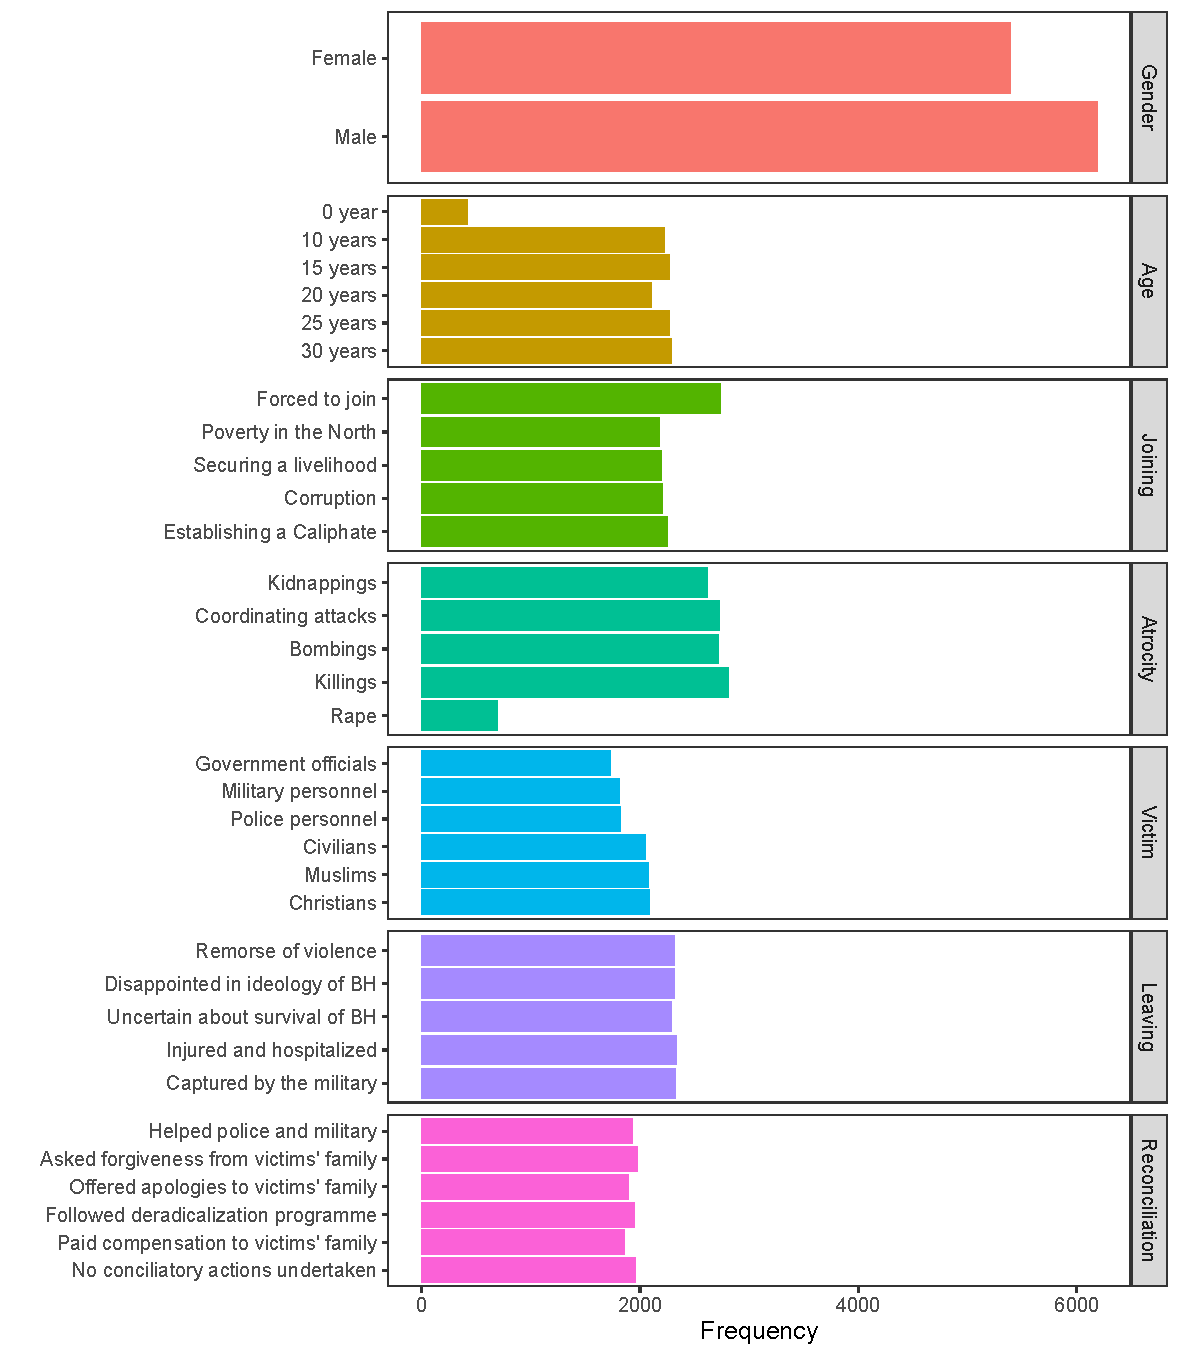
\includegraphics[scale=0.65]{Appendices/Appendix_chapter_3/art2-app-figure4.pdf}
\caption{Frequencies}
\label{fig:art2-app-fig4}
\end{figure}

%~~~~~~~~~~~~~~~~~~~~~~~~~~~~~~~~~~~
\newpage
\subsection{Balance Tests for Covariates Used}
%~~~~~~~~~~~~~~~~~~~~~~~~~~~~~~~~~~~
In Figure \ref{fig:art2-app-fig5}, we test whether the randomization procedure produced experimental groups that are well-balanced across the covariates used in the main article. We test this by regressing respondents' religious background, exposure to Boko Haram violence, and anger reactions to Boko Haram violence against the profile features. The confidence intervals hover closely around the grand mean which suggests little to no imbalance. 
\vspace{3mm}

\begin{figure}[H]
\centering
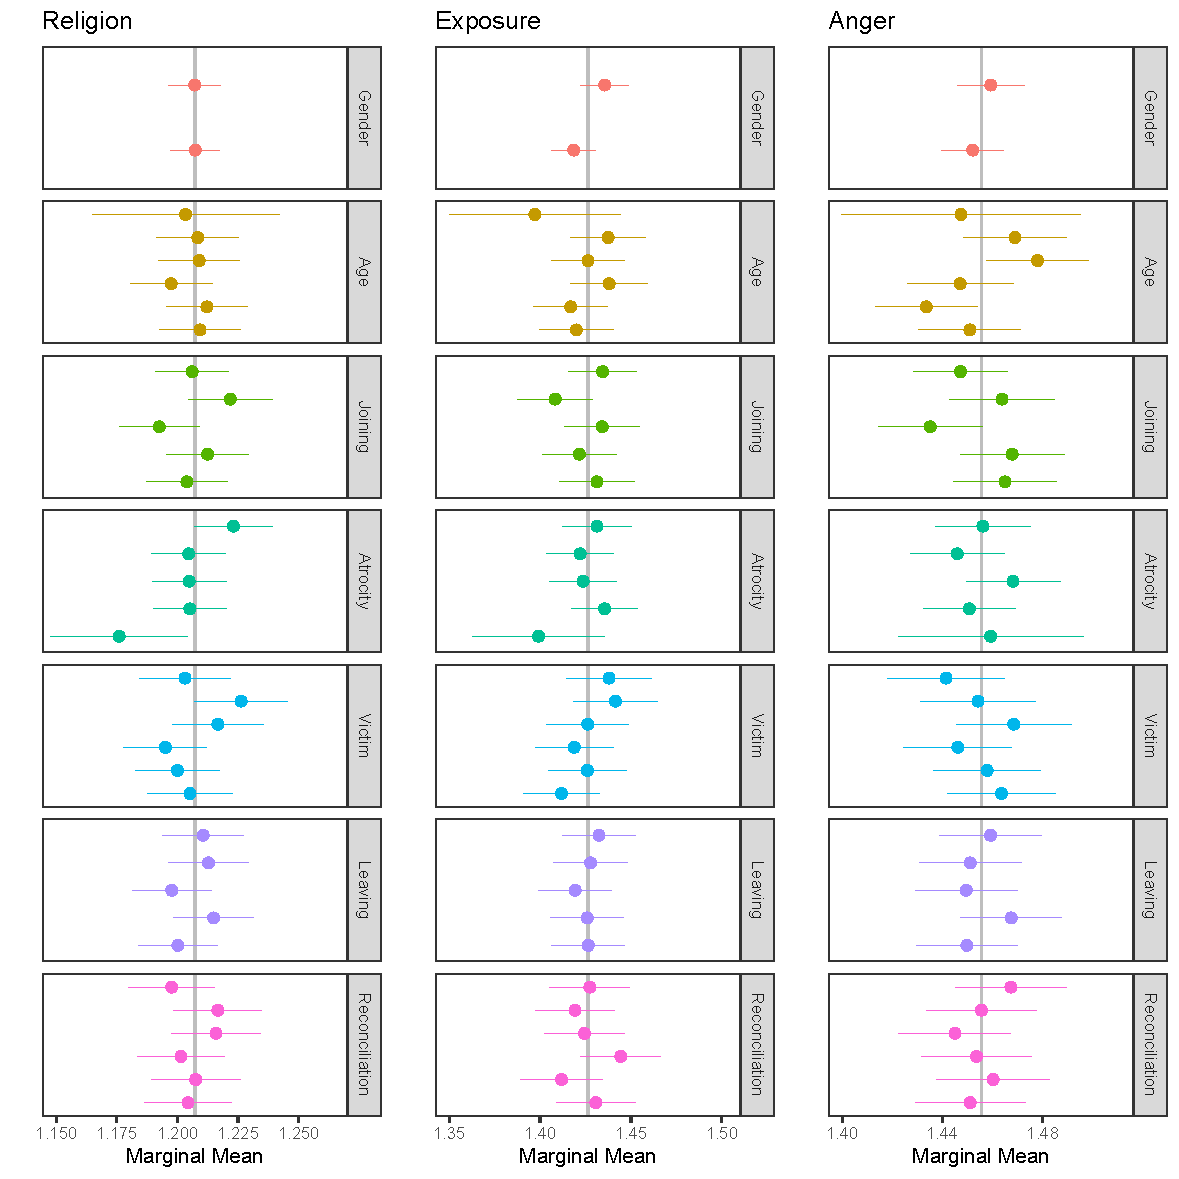
\includegraphics[width=\textwidth]{Appendices/Appendix_chapter_3/art2-app-figure5.pdf}
\caption{Balance Test for Covariates}
\label{fig:art2-app-fig5}
\end{figure}

%~~~~~~~~~~~~~~~~~~~~~~~~~~~~~~~~~~~
\newpage
\subsection{Carryover and Left/Right Assumption Tests}
%~~~~~~~~~~~~~~~~~~~~~~~~~~~~~~~~~~~
One of the assumptions underlying conjoint analyses states that ``the potential outcomes always take on the same value as long as all the profiles in the same choice task have identical sets of attributes'' \citep[][p. 8]{Hainmueller2014}. We therefore evaluate whether there the task round or profile placement affect the quantities of interest for both the choice- and rating-based outcomes. Table \ref{tab:art2-app-tab7} below indicates that there are no carryover problems, but that the the left/right placement affects the results of the choice-based design. Figure \ref{fig:art2-app-fig6} reveals that respondents are, on average, more likely to select the left profile, but this does not alter the substantive results of the paper (i.e., the patterns of preference and, especially, the causal AMCE-results remain robust).

\vspace{3mm}
\begin{table}[H]
\setstretch{1.5}
\caption{Assumption Tests}
\label{tab:art2-app-tab7}
\begin{tabular}{@{}p{0.3cm}p{4cm}p{2cm}p{2cm}@{}}
\toprule
\midrule
                          & & F-value & p-value \\ \midrule
\multicolumn{2}{l}{Carry-over assumption}    & &                  \\ 
    & Choice-Based            & 1.0955          & 0.2833               \\ 
    & Rating-Based            & 1.1800          & 0.1578                \\ 
\multicolumn{2}{l}{Left/Right assumption}       & &                \\ 
    & Choice-Based            & 1.7156          & 0.0004                   \\ 
    & Rating-Based            & 0.8778          & 0.7417              \\ \midrule \bottomrule
\end{tabular}
\end{table}

\newpage
%----------------------------------------------------------
% Figure C.6
%----------------------------------------------------------
\vspace{3mm}
\begin{figure}[H]
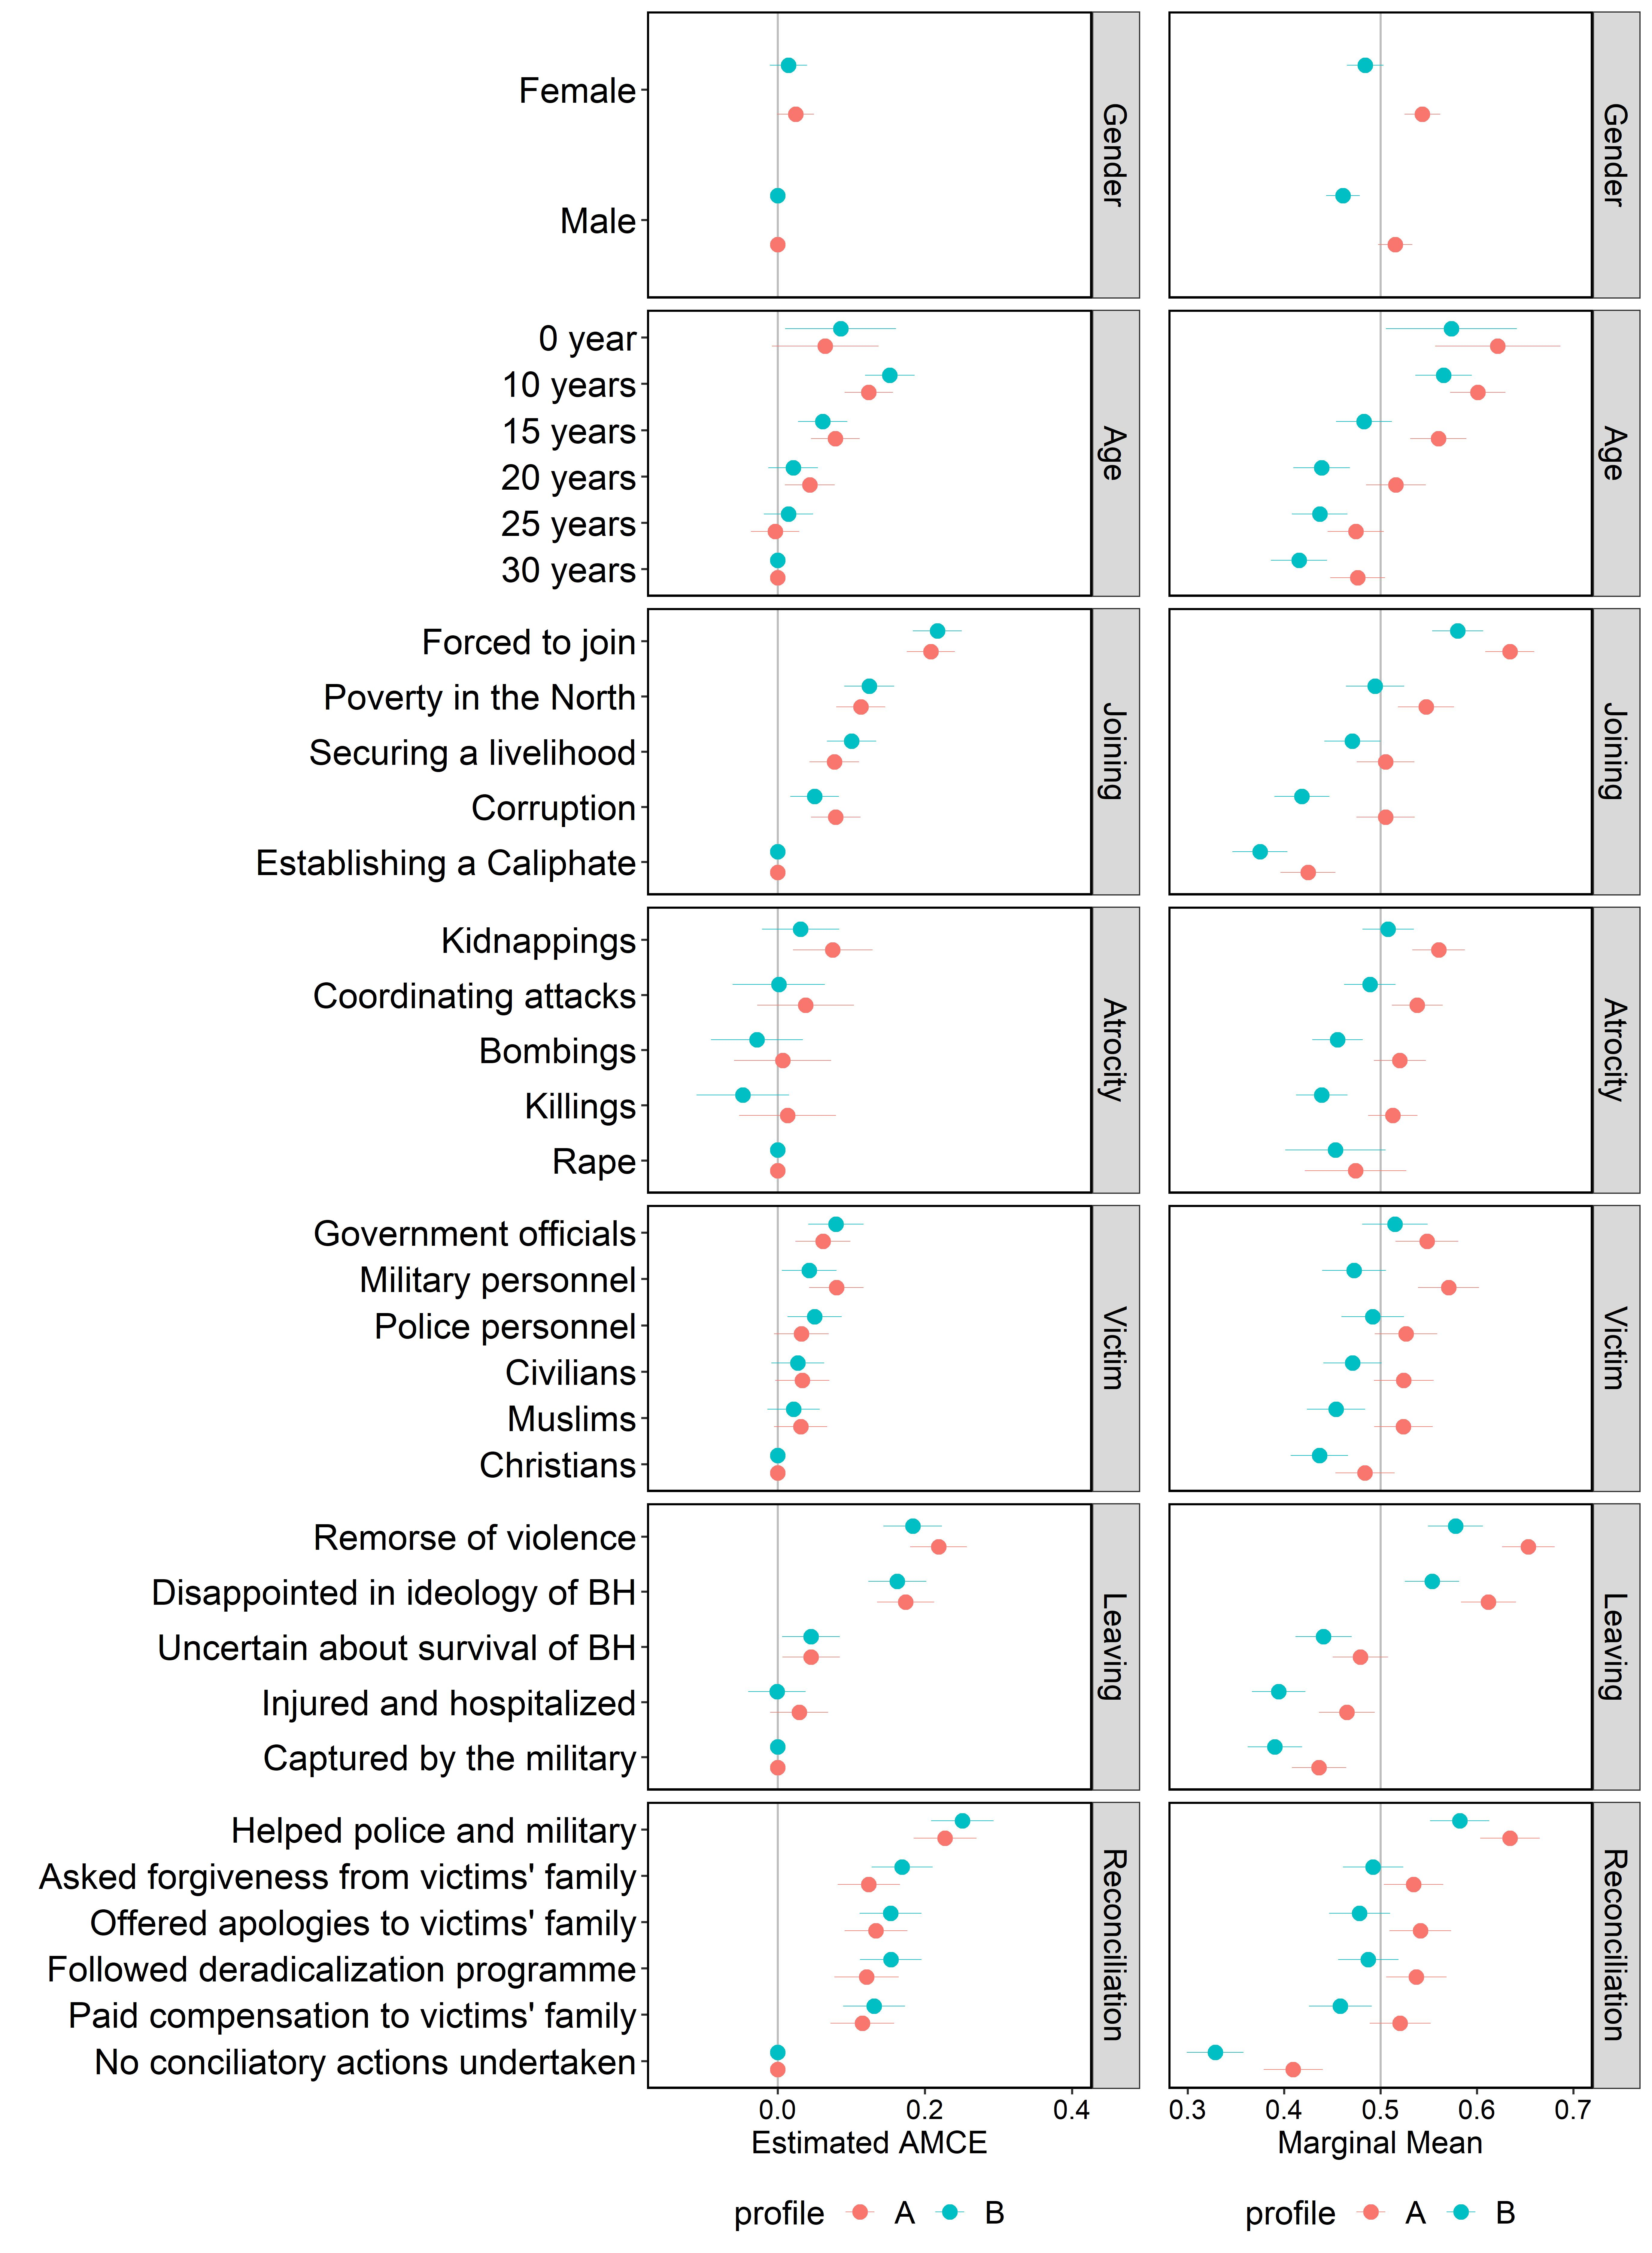
\includegraphics[width=\textwidth]{Appendices/Appendix_chapter_3/art2-app-figure7.jpeg}
\caption{Left/Right Assumption Test for Choice-Based Design}
\label{fig:art2-app-fig6}    
\end{figure}
%----------------------------------------------------------

